\documentclass[sigchi, review]{acmart}
\usepackage{booktabs} % For formal tables

\usepackage[utf8x]{inputenc}
%\usepackage{flushend}
\PrerenderUnicode{aâîțșĂÎÂȚȘ}

% Copyright
%\setcopyright{none}
%\setcopyright{acmcopyright}
%\setcopyright{acmlicensed}
\setcopyright{rightsretained}
%\setcopyright{usgov}
%\setcopyright{usgovmixed}
%\setcopyright{cagov}
%\setcopyright{cagovmixed}


% DOI
\acmDOI{10.475/123_4}

% ISBN
\acmISBN{123-4567-24-567/08/06}

%Conference
\acmConference[AM'17]{AudioMostly conference}{August 2017}{London, UK} 
\acmYear{2017}
\copyrightyear{2017}

%\acmPrice{15.00}


\begin{document}
\title{Soundscape and sound space in the SoundThimble\\ real-time gesture sonification framework}
%\titlenote{Produces the permission block, and
%  copyright information}
%\subtitle{Extended Abstract}
%\subtitlenote{The full version of the author's guide is available as
%  \texttt{acmart.pdf} document}

\author{Grigore Burloiu, Ștefan Damian,\\ Bogdan Golumbeanu}
%\authornote{Dr.~Trovato insisted his name be first.}
%\orcid{1234-5678-9012}
\affiliation{%
  \institution{CINETic UNATC}
%  \streetaddress{P.O. Box 1212}
  \city{Bucharest} 
  \state{Romania} 
%  \postcode{43017-6221}
}
\email{gburloiu@gmail.com}

\author{Valentin Mihai}
\affiliation{%
  \institution{University "Politehnica" Bucharest\\
  	Faculty of Electronics, Telecommunications and IT}
%  \streetaddress{P.O. Box 1212}
  \city{Bucharest} 
  \state{Romania} 
}
%\email{webmaster@marysville-ohio.com}


\begin{abstract}
We introduce \textit{SoundThimble}, a platform for sonic interaction based on the relationship between human motion and virtual objects in 3D space.

A Vicon motion capture system and custom software are used to track, interpret and sonify the movement and\linebreak gestures of a performer relative to a virtual object.

We define three possible interaction dynamics, centred around object searching, manipulation and arrangement. We illustrate the resulting possibilities for layered structures and extended perception and expression.

The software developed is open source and portable to similar hardware systems, leaving room for further extension of the interaction mechanics.
\end{abstract}

%
% The code below should be generated by the tool at
% http://dl.acm.org/ccs.cfm
% Please copy and paste the code instead of the example below. 
%
\begin{CCSXML}
 <ccs2012>
 <concept>
 <concept_id>10010405.10010469.10010475</concept_id>
 <concept_desc>Applied computing~Sound and music computing</concept_desc>
 <concept_significance>500</concept_significance>
 </concept>
 <concept>
 <concept_id>10003120.10003121.10003128.10010869</concept_id>
 <concept_desc>Human-centered computing~Auditory feedback</concept_desc>
 <concept_significance>300</concept_significance>
 </concept>
 <concept>
 <concept_id>10003120.10003121.10003128.10011755</concept_id>
 <concept_desc>Human-centered computing~Gestural input</concept_desc>
 <concept_significance>300</concept_significance>
 </concept>
 <concept>
 <concept_id>10010147.10010178.10010224.10010226.10010238</concept_id>
 <concept_desc>Computing methodologies~Motion capture</concept_desc>
 <concept_significance>300</concept_significance>
 </concept>
 </ccs2012>
\end{CCSXML}

 \ccsdesc[500]{Applied computing~Sound and music computing}
 \ccsdesc[500]{Computing methodologies~Motion capture}
 \ccsdesc[300]{Human-centered computing~Gestural input}
 \ccsdesc[300]{Human-centered computing~Auditory feedback}

% We no longer use \terms command
%\terms{Theory}

\keywords{Sonification, motion capture, gesture spotting, interactive installation, soundscapes}


\maketitle

\section{Introduction}

High resolution three-dimensional motion tracking is traditionally used for animation in film and games, as well as for life sciences research and engineering applications~\cite{welch2002motion}. This technology has long been mined by the audio computing community, although in many early cases, technical limitations meant that the motion data transmission and the sound generation processes were not simultaneous~\cite{dobrian2003gestural, kapur2005framework}.


The \textit{SoundThimble} project harnesses current motion capture technology and gesture detection algorithms to enable new modes of real-time sound exploration and transformation. Our aim is to push beyond the standard paradigms of isolated body motion audification~\cite{dobrian2003gestural,kapur2005framework} or sound control interfaces~\cite{eckel2009motion}, towards deeper narrative structures coupled with layered arrangement of sonic patterns. The result is a platform for interactive sound installations, dynamic composition and augmented dance performance.


Our implementation uses a state-of-the-art Vicon motion capture system\footnote{See  \url{https://www.vicon.com}.} containing eight Vantage 5-megapixel infrared cameras and two Bonita video cameras. Since the open-source software developed in this project\footnote{Available at  \url{https://github.com/RVirmoors/viconOSC}.} is built around Vicon's Datastream SDK,\footnote{See  \url{https://www.vicon.com/products/software/datastream-sdk}.} the platform can be ported to both older and future Vicon-based systems.

In the remainder of the paper, we review relevant literature and technology (section~\ref{sec:related}), we describe the general \textit{SoundThimble} concept and its implementation in an installation (sections~\ref{sec:proj},~\ref{sec:implem}), and finish with a survey of future challenges and perspectives (section~\ref{sec:conc}).

\section{State of the Art}
\label{sec:related}

Sonification, as the auditory representation of a datastream, is a rich tool for translating human movement~\cite{hermann2011sonification}. From a music perspective, infrared motion capture systems have been revealed as a technically superior means for expressive interaction in a controlled environment, with many features being translatable to more portable technologies~\cite{skogstad2010using,vigliensoni2012quantitative}.

In particular, Vicon motion capture systems have been used for over a decade for music applications~\cite{dobrian2003gestural,kapur2005framework,eckel2009motion,vigliensoni2012quantitative}.\linebreak A software bridge for streaming OSC data from Vicon \linebreak exists\footnote{See \url{http://sonenvir.at/downloads/qvicon2osc/}.}~\cite{eckel2009motion} as part of a concluded project, which proved to be incompatible with our current setup.

This decade has seen qualitative advances in the interaction between human gesture and sound behaviour, made possible by real-time gesture recognition and following tools~\cite{caramiaux2014mapping,caramiaux2015adaptive,probabilisticmodels}. These allow for more complex scenarios, where movement is used both for direct sonification and for multi-level control of system behaviour---features which our project channels into a coherent framework.

\section{Concept}
\label{sec:proj}

% inovare = abordarea spatializarii obiectelor sonore / acusmatics

The ``sound-thimble", as the basic building block of our framework, is based on the concept of \textit{sound object} in the Schaefferian sense, as a clearly delimited sounding unit, open to manipulation, arrangement and composition~\cite{schaeffer1998solfege}.

Such an entity, once instanced, can retain an ambiguous nature (spatially and acousmatically) or can switch to a more material state (positioned in space and tied to a causal source)~\cite{soundunseen}. The duality between the latent positioning of the object (which can be inferred from phenomena other than spatial sound reproduction), and the active sound spatialisation and transformation, becomes an innovative tool for the sonic arts, by enabling sound sketching, auditory games and other real-time sound interactions. 

\subsection{Interaction scenario}
\label{sec:scenario}

We present an initial application of our framework, in the form of an interactive installation comprising three phases: search, manipulation, arrangement---corresponding to\linebreak schemas of play, performance, and composition, respectively.

The narrative begins as an immersive game, with a human player attempting to find a sound-thimble (a stationary virtual object, randomly positioned in 3D space), by analysing cues that are constantly shifting in the sonic fabric based on the hand's movement relative to the object. Analogously to the traditional game of \textit{Hunt the Thimble} (a.k.a \textit{Hot or Cold}), the space between the human and the virtual object is correlated to dynamic sound generation parameters, guiding the player's hand towards its target.

Once the object is found it attaches to the hand, and its sonic manifestation gains a richer causal relationship: the player becomes a performer, and is now able to explore the object's sonic palette, and record a number of gestures that can be re-performed later, re-called, and used to trigger or manipulate sonic shifts and events.

Finally, the human can place the virtual object on the floor, or discard it by ``pushing" it outside of the installation boundaries. This triggers a new object to be randomly generated, while the player retains a degree of control over the initial object by recalling recorded gestures. Both objects are now in a latent state, with the new one guiding the player's search, and the previous one responding to the learned set of gestures.

This repeating scenario is outlined in Figure~\ref{fig:concept}. %: objects are randomly generated, the performer finds them, defines gestures and interacts sonically, before arranging them in a pleasing configuration. 
With each spawning of an object or assignment of a gesture, the game becomes more challenging and complex, but also more flexible and rewarding. A demonstration video of the installation project in its current state is available online\footnote{See \url{https://youtu.be/K2Xni2lWswg}.}.


\begin{figure}[t]
	\centering
	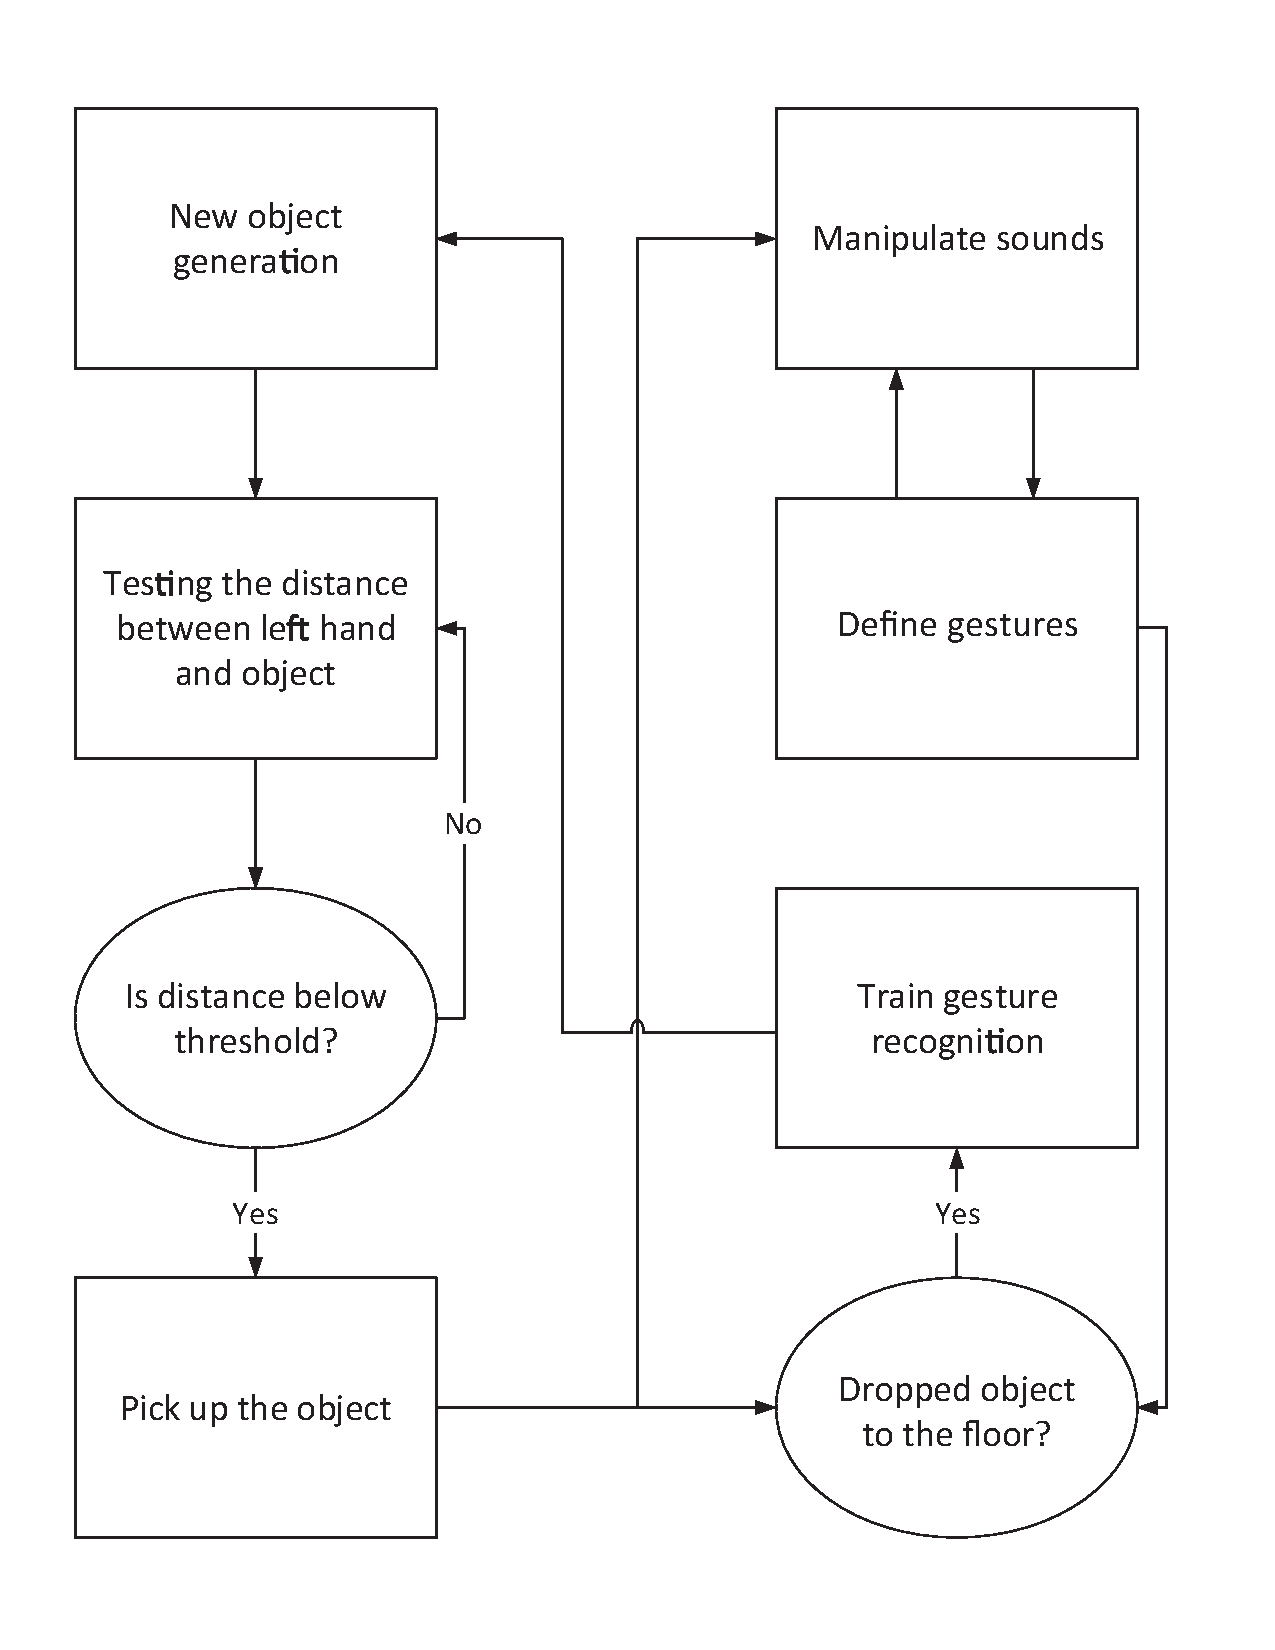
\includegraphics[width=.65\columnwidth, clip, trim={0 .55cm 0 0}]{img/concept}
	\caption{\textit{SoundThimble} interaction workflow.}
	\label{fig:concept}
\end{figure}

\subsection{Performance aesthetic}
\label{sec:aesthetic}

The human-object dynamic at the core of our framework results in certain interaction features which circumscribe the aesthetics of any application of the platform, such as the one described above.

Our approach is informed by Worrall's study~\cite{worrall2013understanding}, which reveals a necessity for the mapping of minute gestural inflections to alter sonic material with a view to certain modes of listening. The aim of \textit{SoundThimble} is to fluctuate between: reflexive, kinaesthetic, connotative, empathetic, reduced.

The cross-modality between different kinds of sense perception guides the performer's attention to the various sonic responses to physical actions. The multi-modal information is processed in real time, continuously redefining the affordances enabled by the system.

Moreover, since the system's responsiveness is reliant on marker visibility, the performer becomes, to a degree, existentially dependent on the camera eye. This, coupled with the coexistence of virtual, responsive objects in the same scene, can lead to novel mechanics at the limits between presence and absence, real and virtual.

\section{Implementation}
\label{sec:implem}

%Many interactions and programable elements which are included in the concept have an exactly function and usefulness. These elements are created in MAX with the help of Vicon SDK and OSC C++ library. The concept suppose an interactive action of a performer or a simple user with an virtual object which has associated gestures defined by person. Virtual object interaction acts in sound design utility like a master controller. Searching for a certain object comes with an audio feedback which makes the search easier.  A dynamic mapping of marker's coordinates is necessary to transfer data between Nexus and MAX.

%One of the first challenges was to create a method of sending real-time from Vicon to MaxMSP where data would be processed and used to generate and manipulate sound. By default, the Vicon system does not support the Open Sound Control (OSC) protocol (ref), needed to communicate with MaxMSP. To overcome this limitation, some code modifications and additions have been implemented inside Vicon’s Blade sdk.

%\begin{figure}[t]
%	\centering
%	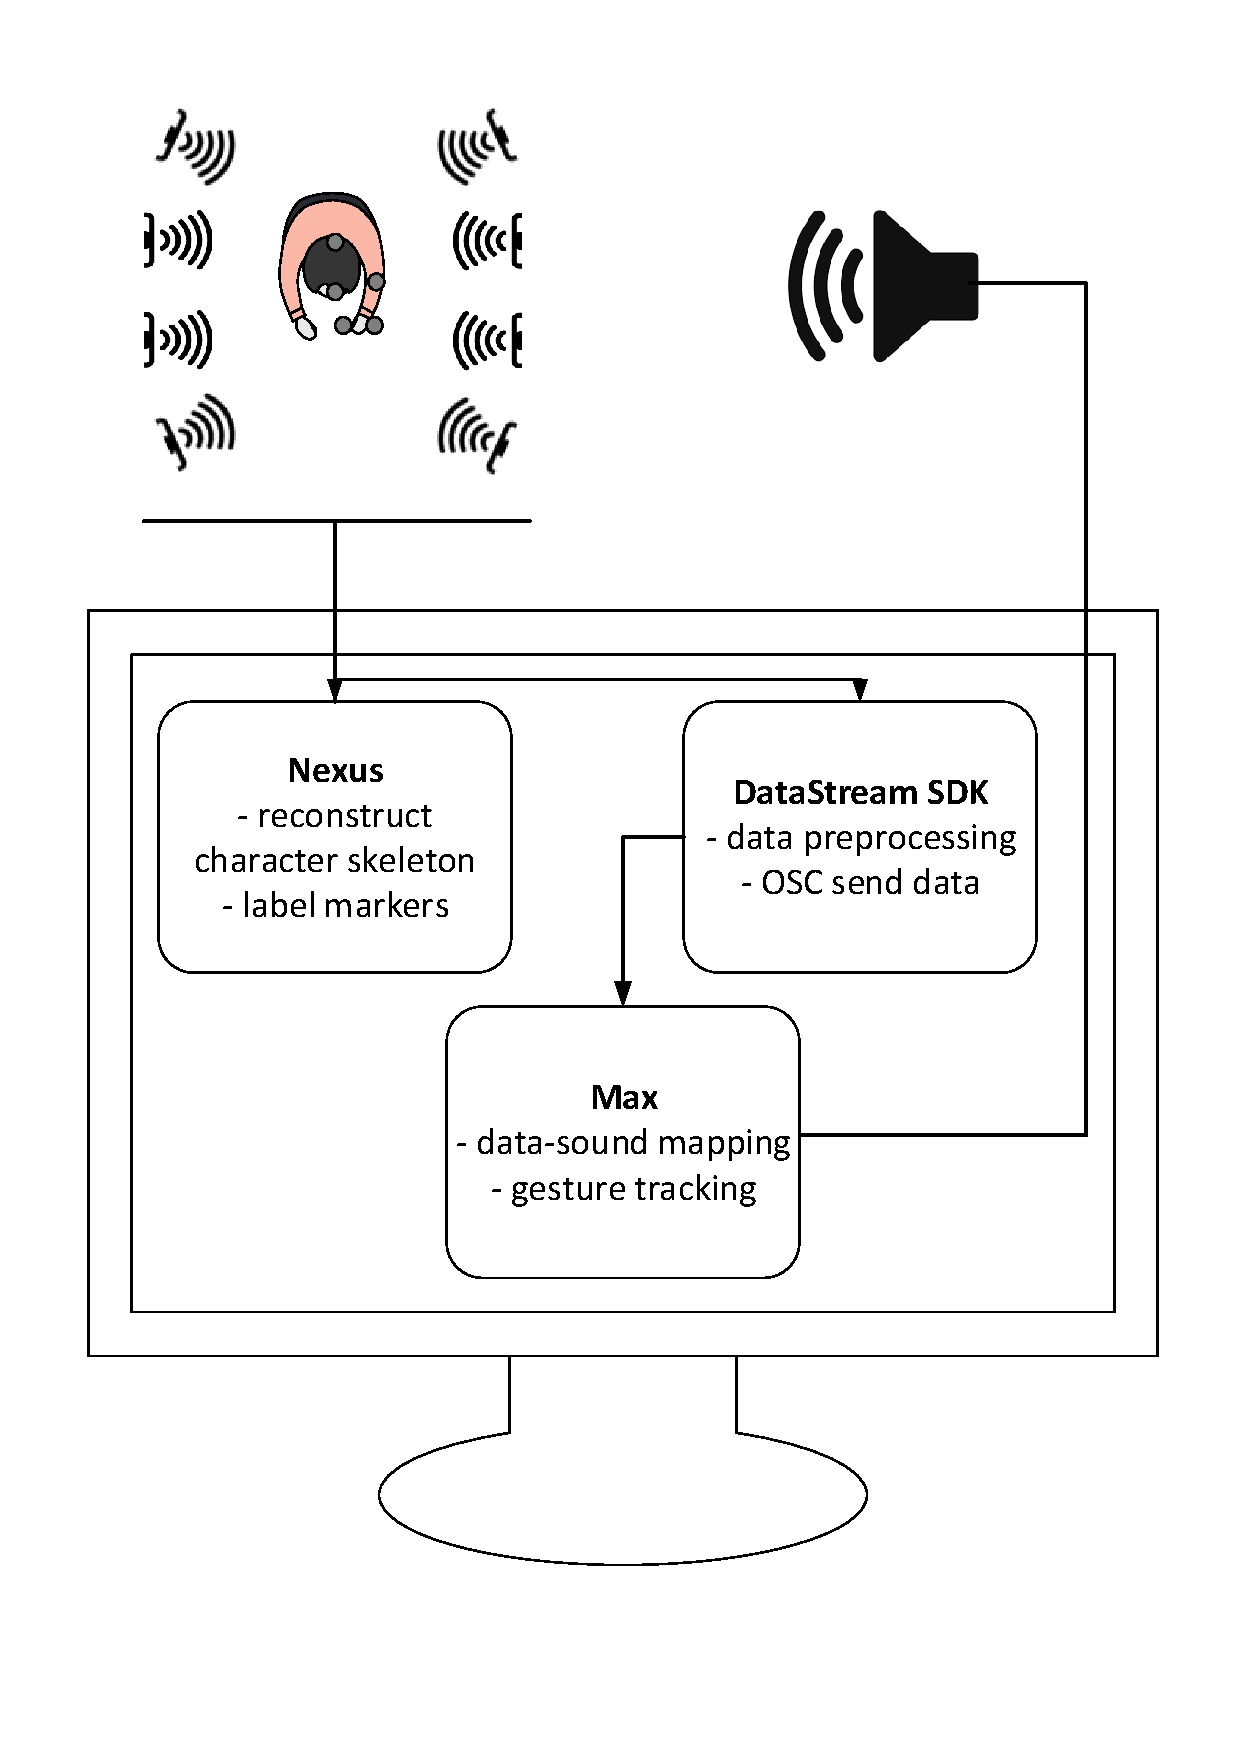
\includegraphics[width=.65\columnwidth, clip, trim={0 3cm 0 0}]{img/archi}
%	\caption{\textit{SoundThimble} framework architecture.}
%	\label{fig:archi}
%\end{figure}

%The framework architecture diagram is laid out in Figure~\ref{fig:archi}. 
Three-dimensional sensor data is streamed into the Vicon Nexus software, which is able to reconstruct and label the underlying character skeleton. The gesture recognition and sonification algorithms are programmed in Max\footnote{Max is a state-of-the-art programming environment for real-time multimedia: \url{http://cycling74.com/}.}, which receives control data via the OSC\footnote{OpenSoundControl is a multimedia communication protocol: \url{http://opensoundcontrol.org/}.} protocol. Since Vicon systems do not support OSC out of the box, we used the \textit{oscpack}\footnote{See \url{http://www.rossbencina.com/code/oscpack}.} library to extend the DataStream C++ SDK and send OSC bundles to Max.

The following description is tailored to our installation application, but any \textit{SoundThimble}-based project will involve similar conditions.

\subsection{Character design}

Figure~\ref{fig:nexus} shows a skeletal reconstruction in the Nexus environment. We pursued a minimal amount of markers, for ease of setup and prototyping. The resulting configuration---sufficient for tracking hand gestures, while ensuring redundancy in case a marker is obscured from the cameras---consists of 5 markers: two positioned on the head, one on the forearm, and two on the hand (thumb and index finger).

\begin{figure}[t]
	\centering
	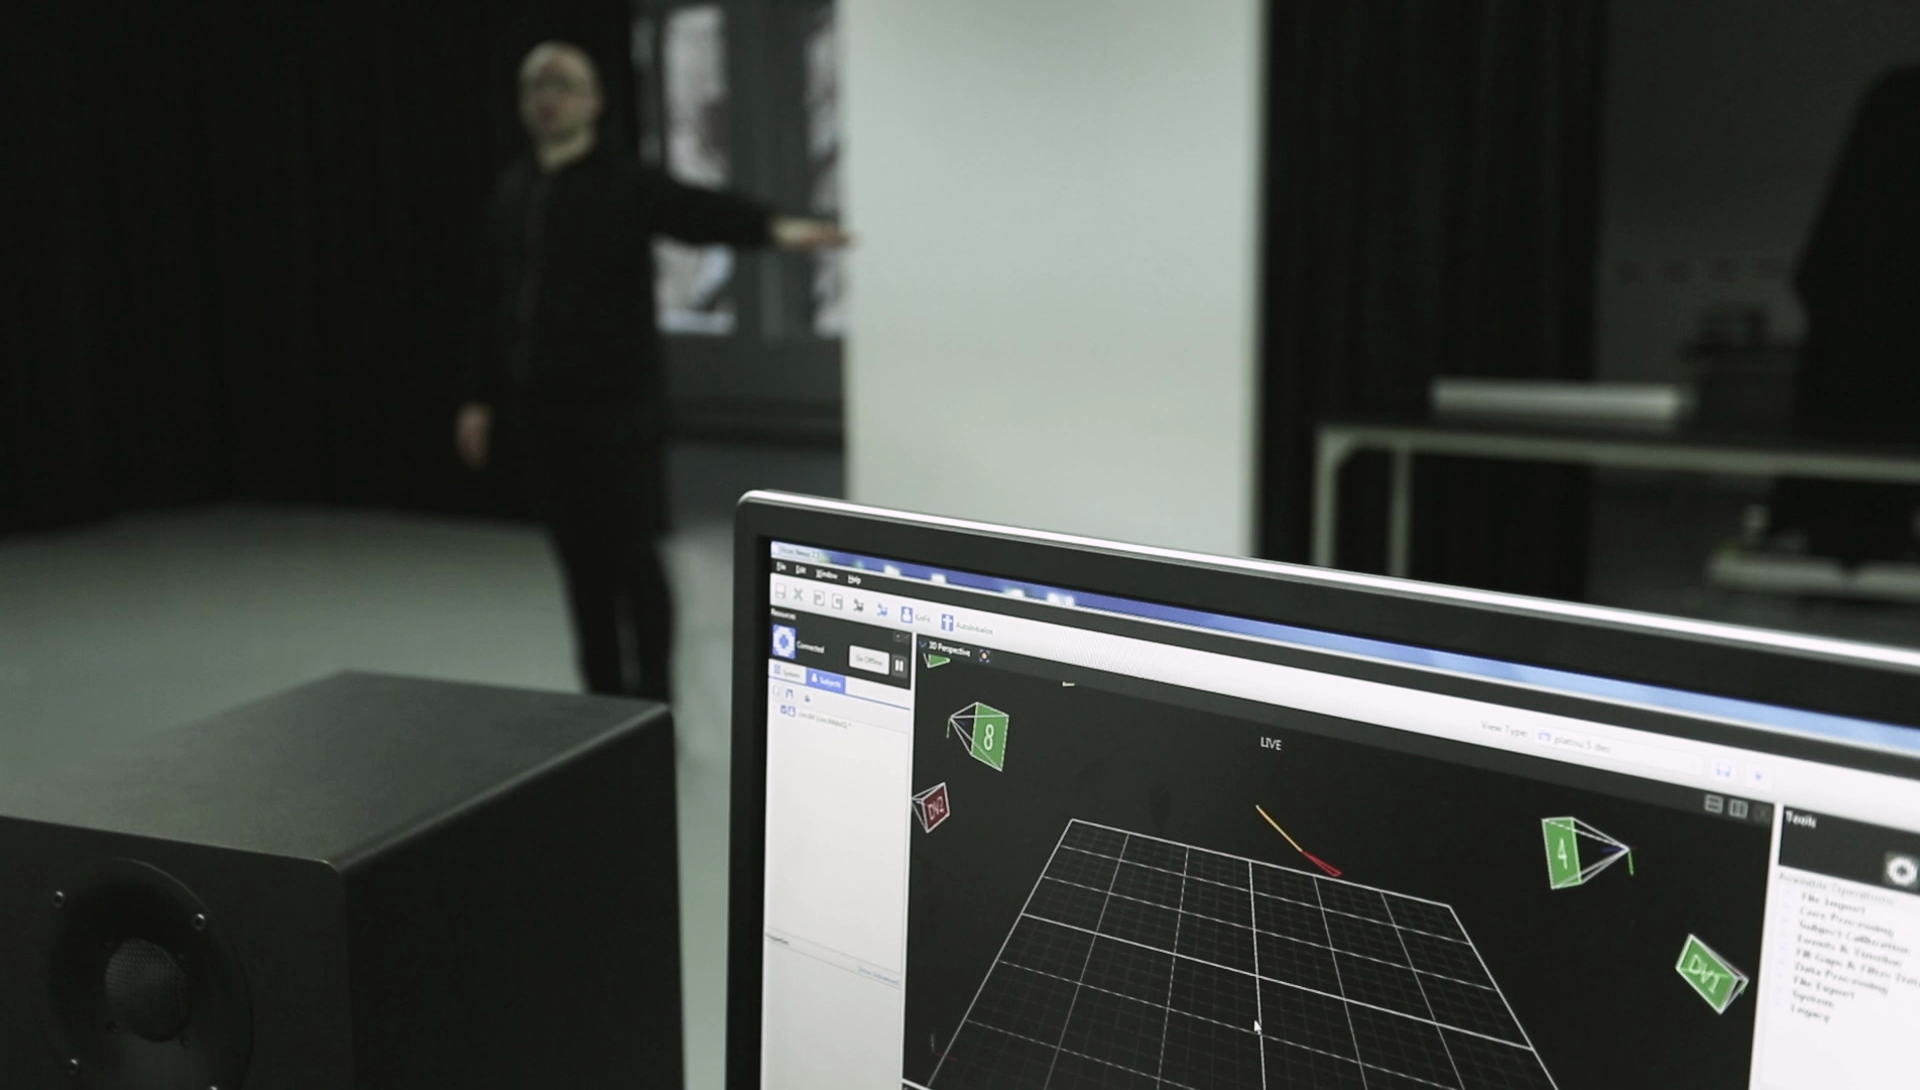
\includegraphics[width=\columnwidth, clip, trim={12cm 0 0 0}]{img/nexus}
	\caption{A performer being tracked in Vicon Nexus. Two visible segments: head-forearm, forearm-hand.}
	\label{fig:nexus}
\end{figure}

Each OSC bundle sent through the SDK consists of the following data:
\begin{itemize}
	\item 3D coordinates for the head (averaged from the two head markers);
	\item 3D coordinates for the hand (averaged from the two hand markers);
	\item distance between thumb and index finger.
\end{itemize}

Each of the three items is sent only if non-zero, i.e. for the head and hand coordinates at least one of the respective markers is active, while for the distance computation, both markers need to be visible and correctly labelled. The forearm marker only serves for skeleton reconstruction, and is not sent via OSC.
%Implementation of the concept presented above requires Nexus, Vicon SDK and MAX sotware. Every character involved in the scene is defined by a limited number of markers. In this case, two markers are positioned on the head, one marker is positioned on elbow and the others 2 on the hand (thumb and index finger). Every marker has associated a name in Nexus and between them 6 segments are drawn. It is very important in realtime capture motion, that the marker to have assigned correct coordinates.
%Also, the Vicon DataStream Software Development Kit (SDK) admits inside changes such as labeling markers, timecode generation and framerate.
To maximise responsiveness and minimise data loss, we raised the frame rate to 500Hz, taking into account the maximum movement speed and the minimum spacing between markers~\cite{song2016fast}. This configuration produces highly stable and responsive inputs into the Max system, with a spatial resolution of 1mm and a latency of around 5ms.

\subsection{Object generation \& interaction mechanics}

The following object-related mechanics are implemented as basic algorithms in Max: generation, detection, release.

Objects are generated at random positions within the boundaries of the motion capture field. Detection of the sound-thimble occurs when the distance between hand and object falls below a set threshold. By default this threshold is set at 200mm radial distance; lowering it can make the game considerably more difficult. Once the object is detected, it becomes mobile, its coordinates tracking those of the hand's.

Finally, a simple thresholding of the $z$-axis (height) value of the hand position serves to release the object. If the velocity computed on the $x$ or $y$ axes (horizontal plane) is high enough, then the object is able to leave the installation space, essentially being removed from the game.
At this point, a new object is generated. The system keeps track of all object coordinates, as they appear and disappear over time.


\subsection{Gesture recognition}

We use the thumb-index finger distance value to enable gesture recording while the two fingers are kept close together. The input features captured into \textit{MuBu} multi-buffer containers~\cite{mubu} consist of cylindrical triplets:
\begin{itemize}
	\item $\Delta \theta / \Delta t$, with $\theta = \tan^{-1}(\frac{y}{x})$;
	\item $r = \sqrt{x^2 + y^2}$;
	\item $z$,
\end{itemize}
where $x$, $y$, $z$ are the respective differences between head and hand Cartesian coordinates, as received via OSC. This feature preprocessing serves two purposes:

Firstly, gestures are recorded based on the position of the hand relative to the head, thus becoming invariable to the performer's absolute \textit{position} within the space. Secondly, by considering the variation of angle $\theta$ over time (as opposed to its absolute value), gestures become invariable to the performer's \textit{orientation} on the horizontal plane. Thus, gestures can be recorded and recalled anywhere within the space, irrespective of the direction the performer is facing.

The input features are fed to the \textit{Gesture Follower} \texttt{gf} Max object, part of the \textit{MuBu} package. The algorithm, based on a Sequential Monte Carlo inference engine~\cite{caramiaux2015adaptive}, allows for \textit{gesture spotting}, i.e. it constantly produces likelihood values of a certain gesture being active, together with an approximation of its completion rate. If these exceed a certain threshold, the respective gesture is triggered. Once detected, the gesture can be followed at a variable rate or scale, even backwards. %The only drawback is that it requires a start trigger, which we send by quickly attaching and separating the thumb and index finger.

Each generated object can have a number of gestures associated to it. When an object is released to the floor, the classifier is (re)trained with the new data, and consequently gestures can act as on/off switches for a particular sonic behaviour (if they are performed/spotted once at a time), or as continuous controllers (if they are repeated by the performer). When several objects exist in the space, a specific movement might act on one or more objects, depending on which detection likelihoods exceed the threshold. 

%In order to control every generated object, there are associated 2 or 3 gestures saved by the performer, but there is a limited time for the gestures to be executed. Predefined gestures offer the possibility to delete the gesture just saved and also indicate the moment the gesture is recorded.

\subsection{Sound design}


Each sound-thimble has a corresponding sound design Max patch, differing in (a) the source sound material used, (b) the synthesis techniques applied, and/or (c) the control mapping schema to the object search and manipulation variables. The various combinations of (a), (b) and (c) give rise to a growing library of objects, each with its own character. By designing various interaction rules for each object, they are linked to spatially aware parameters adding up to a continuously evolving, organic soundscape.

%We differentiate between the three phases of the installation in terms of mapping technique and level of sonic interactivity. The search mode employs straightforward parameter mapping, where human-object distance measures are linked to synthesis parameters, while the manipulation phase relies on a model-based mapping approach where different gestures and actions reach deeper levels of control~\cite{hermann2011sonification}. Finally, variations on both these techniques occur in the arrangement phase.

%The synthesis patches used for search are built around a process of decorrelation~\cite{kendall1995decorrelation}: the farther the human's hand from the object the more decorrelation occurs, up to the point where each instance of the signal becomes a distinct sonic entity. This is done by continuously modulating each of the copies in terms of pitch (FM) and amplitude (AM) with low frequency oscillators (LFO’s). Changes in frequency, amplitude and wave shape of the LFO’s lead to complex sonorities ranging from coupled streams of sound to distinct iterations with a high degree of randomness. %By moving and assessing sonic shifts and the level of decorrelation, the performer is able to intuitively find the object. 
%This mechanism is subtly mixed with a granular engine in a latent state, which gains more prominence in the next mode.

%In the manipulation phase, the 3D space is split into chunks, each one acting as a zone with its own mappings and interaction laws. The synthesis patches are based on the segmentation of a source sound into short grains. We built a granular synth with these controllable parameters: grain size, grain position, envelope shape, level of scattering, pitch, timbre and stereo width. Another patch implements a concatenative synth that traverses the grains guided by movement velocity and trajectory. Certain gestures trigger sonic events while interpolating between sets of parameter values via a convergent-mapping schema~\cite{hunt2000mapping}. %This patch is active in both the object search and manipulation phases, differing between them in the dimensionality of control and presence in the auditory scene. 
%In order for the user-experience to be truly engaging, a great deal of calibration needs to be done in respect to the physical space. This is done by setting and tweaking ranges, scaling laws, assigning thresholds and designing various function curves.


%In the search phase, all sound design is based on two channels that can either be routed to multiple pairs of speakers or downmixed to mono and diffused on an arbitrary number of speakers. In the manipulation phase, the soundscape is spatialised to track the position of the performer. In the arrangement phase, the dropped object retains a ``root" source location, which can relate dynamically to the performer position when a gesture is executed: for instance, the granular patch sends spatialised grains back and forth between the dropped object and the performer.

In addition, we enable the definition of "hotspots" in 3D space, each acting as a zone with its own mappings and interaction laws. A higher resolution of hotspots allows for more detailed design schemas.


For developing sonification algorithms, we provide two input data sources. The first one is motion capture data recorded via Nexus into MuBu containers. For more flexibility and immediate control, we also created a basic visual interface to monitor the input data and to manipulate it in virtual 3D space using the mouse, for instant auditory feedback. This feature comes in useful when specific motion data is not available and needs to be roughly simulated.

%\section{Case studies}
%\label{sec:case}
%
%We present two applications of our platform: a participative installation, and a performance piece. They represent two manifestations of the \textit{SoundThimble} concept and infrastructure, revealing a pair of experiences: (a) the direct interaction with sound in space, and (b) the mediated interaction with sound and space of an audience member. In both cases, the range of sense and perception is extended through new experiences.
%
%
%\subsection{Interactive installation}
%
%The first form conceived for the \textit{SoundThimble} platform is that of an open installation, where visitors become participants and observers in the situation outlined in section~\ref{sec:scenario}.
%
%Beyond the considerations in section~\ref{sec:aesthetic}, the major feature of the auditory game is the layered sequence of search-manipulation-arrangement which translates to a layering of awareness of accumulated experiences. The meshing of sound objects (supplied by the game) and gestures (defined by the player) leads from a state of uncertainty and potential, to phases of exploration, play, composition. Snapshots of interest can be stored for later recall---currently this is done manually, but might be automated in the future.
%
%\subsection{Dance performance}
%
%The following is a sketch for a work currently under development. A performer enters the motion capture space, and commences a series of improvised motions, silently establishing the action space.
%
%Once a threshold is reached, a virtual object is generated and the movement is no longer completely free, its range of action being directed by the relationship to the object position. Searching and finding the sound-thimble is a process of correlating the sonic characteristics to one's own movement patterns.
%
%By ``resonating" with the object's manifestation and locating it, the performer enters the manipulation phase, extending her auditive and tactile perception through embodied listening. The multimodal information processed by the performer is both cochlear and kinaesthetic/proprioceptive, tactile, vestibular and visual. Thus, the information she forms about the shape of the movement, its trajectory and spatial dynamics, is intrinsically linked to the sonic connections to these parameters. This dynamic knowledge influences the timing of new actions and the anticipation of sonic feedback. The resulting action schemas are composed as both spatial and sonic shapes.
%
%Gradually, as the performer's control patterns become crystallised, the sonic nature of the source object moves between the abstract and the concrete. In the latter phase, the performer is able to control higher-level parameters such as tempo and orchestration of a coherent musical structure which was partly a result of the generative interaction in the more abstract/exploratory phase.



\section{Conclusions and Future Work}
\label{sec:conc}

This paper introduced \textit{SoundThimble}, a multi-layered platform for real-time motion-music interaction.
All the developed software (including the C++ code for data preprocessing and transmission, and the Max patches for gesture tracking and sound design) is open source and publicly available.

The team is currently pursuing several directions for evaluation and extension. While informal tests have been positive, we are also conducting systemic assessments in preparation for the first public installation later this year. Moreover, we plan to support more than one participant at once, implementing mechanics for sharing control of the virtual object. %Video projection support is planned, e.g. each object having a corresponding reactive video, with the arrangement phase also producing a background visual collage. We are also considering eye tracking technology to enable an audience member's active involvement in shaping the sound. 
%Meanwhile, work continues on enriching the interaction and sound design.


Finally, we are commencing the outreach to composers, artists and creative programmers, to apply our platform to new innovative projects and engage in practice-led research.


\bibliographystyle{ACM-Reference-Format}
\bibliography{sonif-ref} 

\end{document}
